% This file contains all homework from week 37
% use \section{<name>}  to create a section per homework assignment

\section[Homework 2]{Homework 2: Recursive Make Considered Harmlful}

In this section we'll describe the solutions for the "Recursive Make" problem as originally described in \cite{make_harmful}.
The three main solutions are explained in detail below:
\begin{description}
	  \item[Reshuffle] \hfill \\
	  Manually tweak the order of the modules in the top-level \textit{Makefile}. This is necessary because \textit{make} uses the postorder transversal, see figure \ref{fig:postorder}, but when dividing the DAG into two pieces, \textit{make} is not allowed to do so. The project dictates the order of transversal, but the order is plain wrong.  \hfill \\
	\begin{figure}[H]
		\centering
		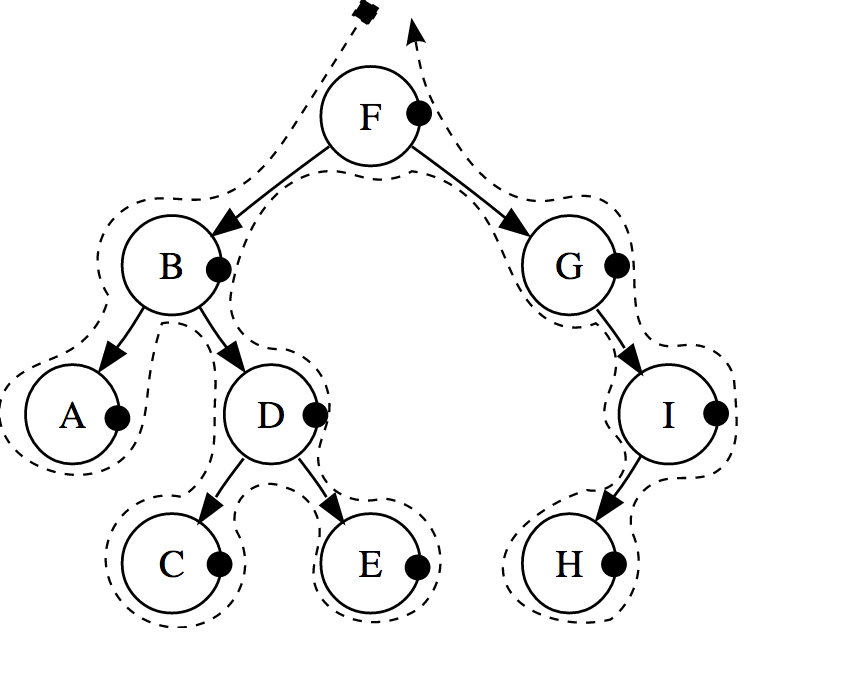
\includegraphics[scale=0.5]{postorder}
		\caption{The postorder traversal the sequence is: A, C, E, D, B, H, I, G, F \cite{postorder}}
		\label{fig:postorder}
	\end{figure}
	  \item[Repetition] \hfill \\
	  This solution tells \textit{make} to make more than one pass in the top-level \textit{Makefile}, an example is shown in script \ref{make_code} \hfill \\
	\begin{lstlisting}[frame=single, language=make, caption={An example Makefile using repetition.}, label={make_code}]
	 MODULES = ant bee 
 	all:
    	for dir in $(MODULES); do \
      		(cd $$dir; $(MAKE) all;) \
    	done
    	for dir in $(MODULES); do \
      		(cd $$dir; $(MAKE) all;) \
    	done 
	\end{lstlisting}
	This will double the time it takes to preform the build. But worse, the upper bound for the number of passes is proportional to the number of graph edges which are linked to multiple modules.
	
	  \item[Overkill] \hfill \\
	As the name suggests, this is like doing to much work. You could threat every dependency as always out of date and thus always - even if nothing changed - rebuilt files with dependencies. This solution will fail in non-deterministic ways when make uses the parallel build option (-j).  
	\end{description}